%!TEX root = slides.tex

\section[Session 2]{Session 2: Empirical methods with which to detect
environmental and phenotypic associations: single and multiple locus
methodologies}

\begin{frame}
\frametitle{Fixed vs random effects}
\begin{block}{Fixed effects}
\begin{itemize}
\item{\textbf{Treatment} effects}
\item{Case vs. control, and \textbf{only} these two groups}
\item{Variable for which all levels are included (e.g., gender, race)}
\item{Explicitly compare between levels without generalizing (e.g., San
Francisco vs. Berkeley)}
\item{Usually qualitative variables}
\end{itemize}
\end{block}
\tiny
\citet{StroupFreund200203}
\end{frame}


\begin{frame}
\frametitle{Fixed vs random effects}
\begin{block}{Random effects}
\begin{itemize}
\item{Drawn from a distribution of possible effects}
\item{San Francisco and Berkeley are just two of many western US, 
or liberal, or hippie, or measels-infected cities}
\item{Use of a random effect allows for more generalizable conclusions 
from the data}
\item{rather than comparing among levels for an effect, random 
effects measure how much variance in the dependent variable is 
accounted for across levels of the random factor}
\item{Blocking, control, repeated-measures factors are random}
\end{itemize}
\end{block}
\tiny
\citet{StroupFreund200203}
\end{frame}



\begin{frame}
\frametitle{Detecting and dealing with population structure}
\begin{block}{Why is this important?}
\begin{itemize}
	\item{Can lead to spurious associations if not accounted for}
	\item{Population structure can look like LD}
	\item{Substantial and varying LD present in genome-scale datasets}
	\item{Which markers to use to access structure? - all of them}
	\item{Leave-one-out testing?}
\end{itemize}
\end{block}
\tiny
\citet{Price:2006cd}
\end{frame}

\begin{frame}
\frametitle{Multiple testing approaches}
\begin{block}{Methods}
\begin{itemize}
	\item Bonferroni
	\item Bootstrapping
	\item FDR
\end{itemize}
\end{block}
\end{frame}

\begin{frame}
\frametitle{Detecting and dealing with population structure}
\begin{block}{}
\centering
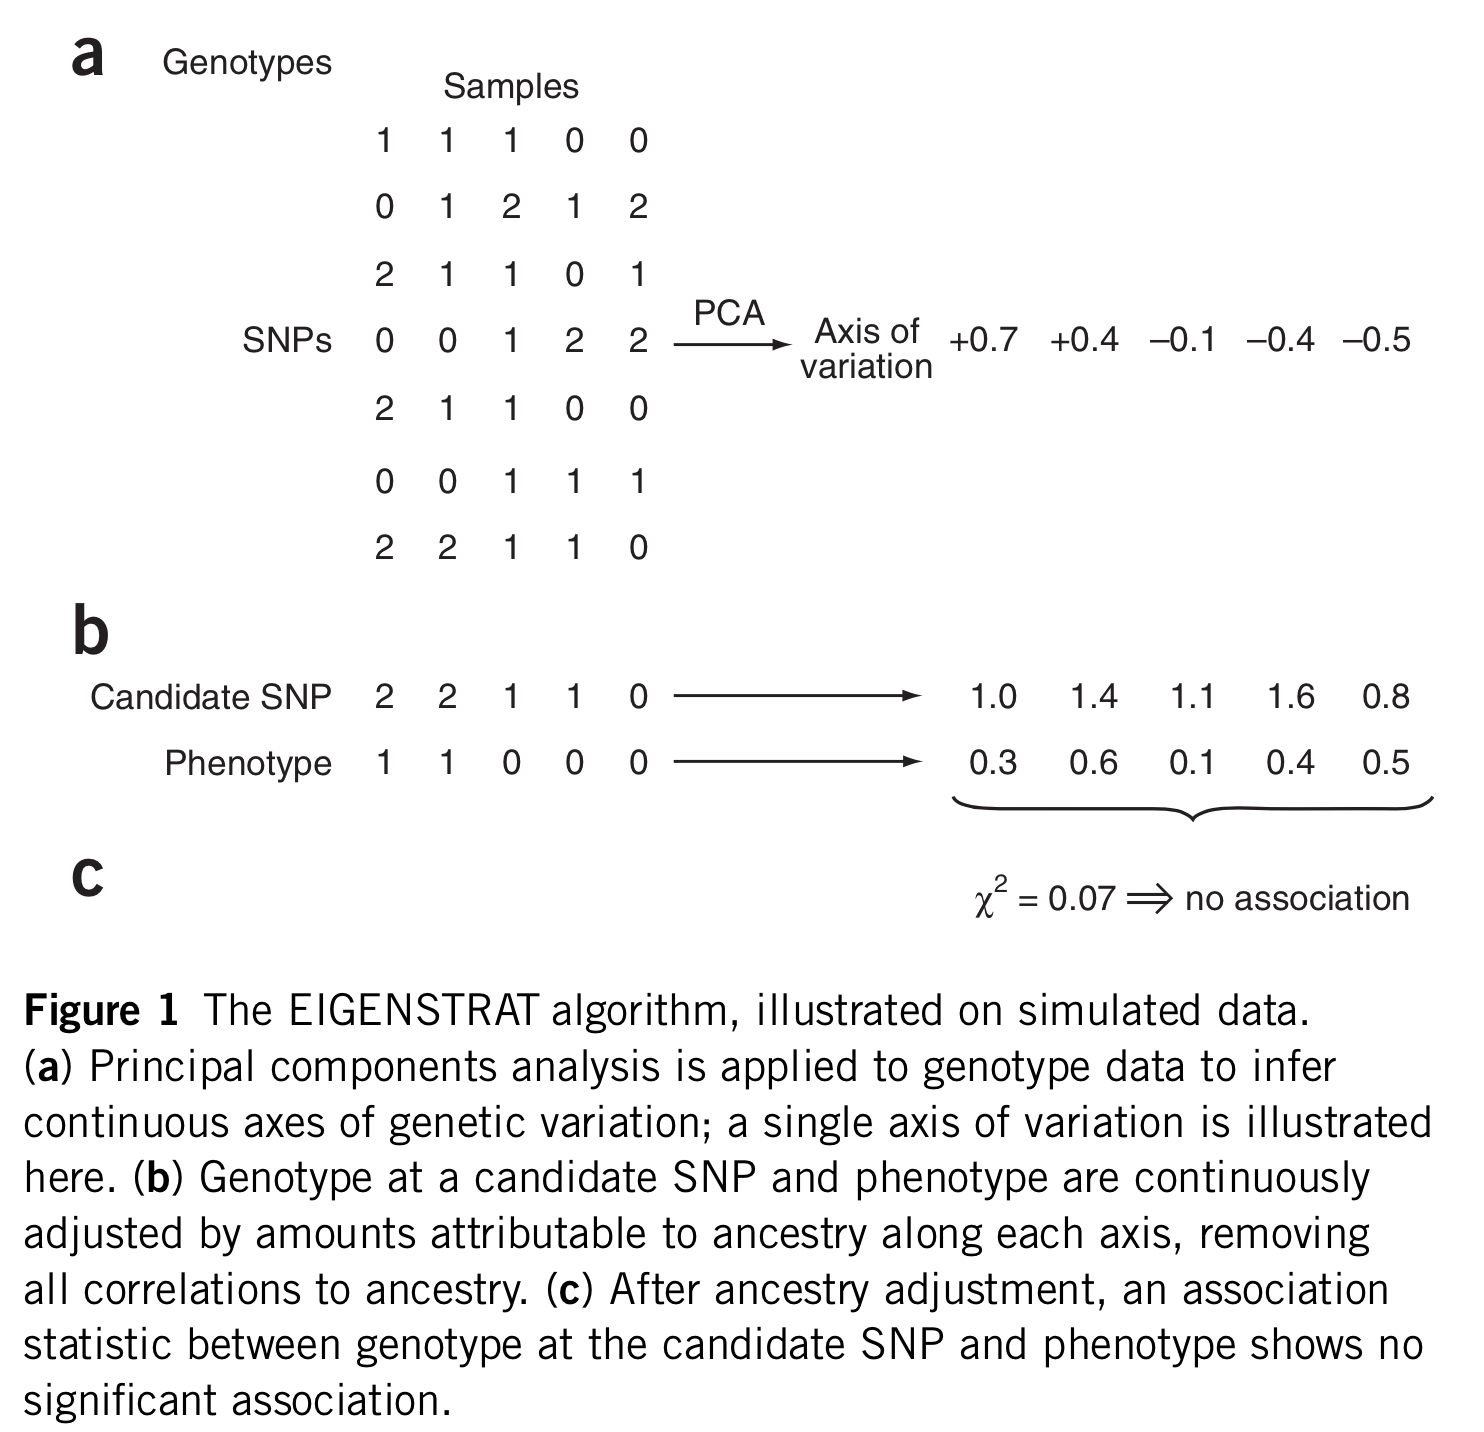
\includegraphics[height=0.8\textheight]{price.png}\\
\tiny
\citet[Figure 1]{Price:2006cd}
\end{block}
\end{frame}

\begin{frame}
\frametitle{Testing SNPs against phenotypes}
\begin{block}{}
\begin{center}
\Large{$y=X \bm{\beta} + S \bm{\alpha} + Q \bm{v} + Z \bm{u} + \bm{e}$}
\end{center}
\begin{itemize}
\item{$X \beta$: fixed effects w/o SNP + population structure}
\item{$\beta$: fixed effects other than SNP or pop. structure}
\item{$\alpha$: vector of SNP effects}
\item{$v$: vector of population effects}
\item{$u$: vector of polygene background effects}
\item{$Q$: matrix from STRUCTURE relating y to v}
\item{$X, S, Z$: incidence matrices (0/1) relating y to $\beta$, $\alpha$, $u$,
respectively}
\end{itemize}
\end{block}
\tiny
\citet{Yu:2006ij}
\end{frame}

\begin{frame}
\frametitle{Testing SNPs against phenotypes}
\begin{block}{}
\begin{center}
\Large{$y=X \bm{\beta} + S \bm{\alpha} + Q \bm{v} + Z \bm{u} + \bm{e}$}
\end{center}
\begin{itemize}
\item{$Var(u) = 2KV_g, Var(e) = RV_R$}
\item{$K$: $n \times n$ matrix of genetic covariance between pairs of
individuals (kinship)}
\item{$R$: $n \times n$ matrix off-diag elems are 0, diag is
$1/N_{{obs}_{pheno}}$}
\item{$V_g$: genetic variance (additive)}
\item{$V_R$: residual variance (non-additive + env)}
\end{itemize}
\end{block}
\tiny
\citet{Yu:2006ij}
\end{frame}

\begin{frame}
\frametitle{Bayenv: identifying correlations with ecological
variables}
\begin{block}{Comparing allele frequencies and the environment}
\begin{itemize}
\item{Given different environments, local adaptation should drive changes in
allele frequencies among populations}
\item{However, allele frequency differences can be artifacts.}
\item{Bayenv (and Bayenv2):}
\begin{itemize}
\item{Accounts for complications due to demography and uneven sampling}
\item{Reports Bayes factors, and correlation statistics for SNPs}
\item{Provides standardized allele frequencies with demographic features
approximately removed, which can be used in other statistical frameworks
to test for environmental correlations}
\item{Bayenv2 can also account for sampling variance in pooled populations}
\end{itemize}
\end{itemize}
\end{block}
\tiny
\citet{Gunther:2013ik, COOP:2010ke}
\end{frame}


\begin{frame}
\frametitle{Bayenv: identifying correlations with ecological
variables}
\begin{block}{Output}
\begin{itemize}
\item{Standardized allele frequencies}
\item{Detect SNP outliers while accounting for population history ($X^TX$)}
\end{itemize}
\end{block}
\end{frame}

\begin{frame}
\frametitle{Bayenv: identifying correlations with ecological
variables}
\begin{block}{}
\centering
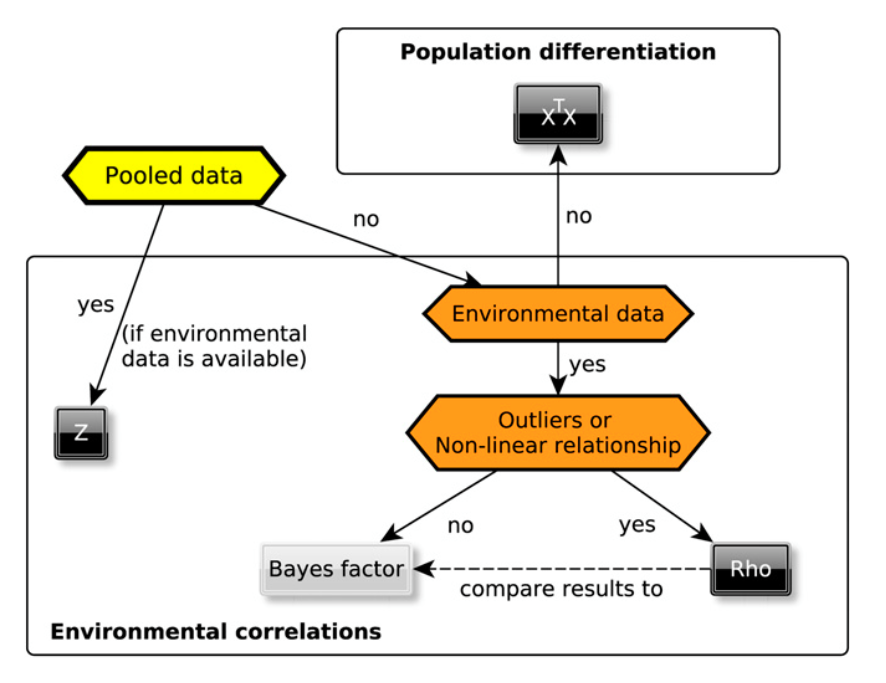
\includegraphics[width=.7\textwidth]{bayenv1}
\end{block}
\end{frame}

\begin{frame}
\frametitle{Bayenv: identifying correlations with ecological
variables}
\begin{block}{The method}
\begin{enumerate}
\item{Estimation of an empirical covariance matrix from allele count data from
L across K populations}
\item{Models joint distribution of allele frequencies across populations}
\begin{equation}
x_{kl} = g(\theta_{kl}) = \begin{cases}
	0 & \theta_{kl} < 0 \\
	\theta_{kl} & 0 \le \theta_{kl} < 1 \\
	1 & \theta_{kl} > 1
\end{cases}	
\end{equation}
\item{Point masses at 0 and 1 represent loss or gain, $\theta_l$ are MVN}

\begin{equation}
	P(\theta_l|\Omega, \epsilon_l) \sim
 N(\epsilon_l,\epsilon_l(1-\epsilon_l)\Omega)
\end{equation}

\end{enumerate}

\end{block}
\end{frame}

\begin{frame}
\frametitle{Bayenv: identifying correlations with ecological
variables}
\begin{block}{The method}
\begin{itemize}
\item{The joint posterior of $\Omega$ over all loci is:}

\begin{multline}
P(\Omega, \theta_1, \ldots , \theta_l, 
\epsilon_1, \ldots , \epsilon_L | 
\bm{n}_1, \bm{m}_1, \ldots , \bm{n}_L, \bm{m}_L) \\
\propto \left \{ \prod_{l=1}^{l=L}P(\bm{n}_l,\bm{m}_l | \bm{x}_l = g(\theta_l))
P(\theta_l | \Omega,\epsilon_l)P(\epsilon_l)
\right \}P(\Omega)	
\end{multline}

\item{This is the null model of SNP frequencies across populations}
\item{Given this model, how are allele frequencies at SNPs correlated with 
the environmental variable(s), $Y$?}

\end{itemize}
\end{block}
\end{frame}































